\documentclass[a4paper, 12pt]{article}
\usepackage[top=1cm, bottom=2.1cm, left=2cm, right=2cm]{geometry}
\usepackage[utf8]{inputenc}
\usepackage{graphicx, caption}
\usepackage{float}
\usepackage{amsmath, amsfonts, amssymb, esint}
\usepackage{hyperref}
\usepackage{multicol}
\usepackage{wallpaper}

\CenterWallPaper{1}{./img/background.png}

\hypersetup{
    colorlinks=true,
    linkcolor=blue,
    filecolor=magenta,      
    urlcolor=cyan,
}

\newcommand{\cabecalho}[4]
{
	\begin{figure}
		\centering
		\href{https://ligaolimpicadeastronomia.com.br/}{
\includegraphics[scale=0.6]{./img/logos.png}}
	\end{figure}
	
	\begin{center}
		\begin{large}
			\textbf{#1}	
		\end{large}
			\linebreak Listas OBA (Nível 4) -- #2ª Lista
			\linebreak #3
		\end{center}
	
	\begin{flushright}
		Material elaborado por \textbf{#4}
	\end{flushright}
}

\begin{document}
	\cabecalho{Questões}{4}{Astronomia de posição}{Iago Braz Mendes}
	
	\begin{flushleft}
	\begin{itemize}
		\item \textbf{Questão 1) (1 ponto)} Na Astronomia de Posição, é muito comum fazer uso do plano altazimutal para estudar os movimentos dos astros. Esse plano se baseia no sistema de coordenadas altazimutais -- Azimute e Altitude (ou Distância Zenital) --, o qual é fixo no observador. Observe o esquema seguinte, o qual reproduz algumas componentes observadas em tal plano:
			\begin{figure}[H]
				\centering
				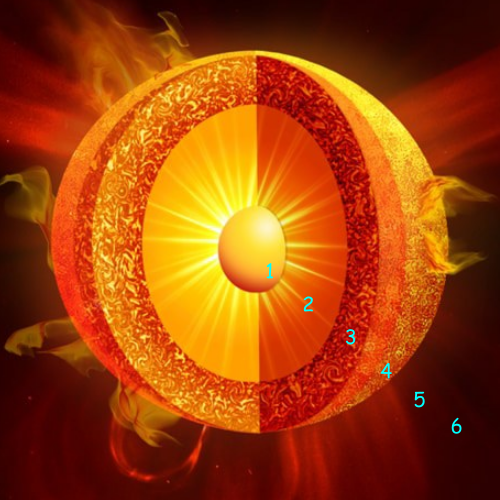
\includegraphics[scale=0.5]{./img/1.png}
			\end{figure}
			em que as letras maiúsculas são pontos e as letras minúsculas representam segmentos de reta (que, na verdade, são a projeção ortogonal das circunferências da esfera celeste na linha de visão). Além disso, semicircunferência em azul é o que o observador pode observar e a em marrom representa a parte da esfera celeste abaixo do horizonte. Por fim, os pontos $PC\_$ representam os polos celestes, sendo que $\_$ pode ser substituído por $N$ (para o Polo Celeste Norte) ou por $S$ (para o Polo Celeste Sul).
			\begin{itemize}
				\item \textbf{Pergunta 1a) (0,4 ponto) (0,1 cada acerto)} Considerando $PC\_$ como $PCS$ para o ponto superior e como $PCN$ para o ponto inferior na imagem, coloque as letras $A$, $B$, $C$, e $D$ (representando os pontos indicados com essas letras no esquema) nas correspondentes nomenclaturas.
					\begin{multicols}{3} \begin{itemize}
						\item[$(\quad)$] Ponto Cardial Norte
						\item[$(\quad)$] Ponto Cardial Leste
						\item[$(\quad)$] Ponto Cardial Sul
						\item[$(\quad)$] Ponto Cardial Oeste
						\item[$(\quad)$] Zênite
						\item[$(\quad)$] Nadir
					\end{itemize} \end{multicols}
				\item \textbf{Pergunta 1b) (0,6 ponto) (0,2 cada acerto)} Agora, coloque as letras $a$, $b$, e $c$ (representando as circunferências indicadas com essas letras no esquema) nas correspondentes descrições. \linebreak
					\textbf{Dica:} a declinação de astros no Hemisfério Norte e Sul é positiva e negativa, respectivamente, e pode ser pensada como similar à latitude, porém na Esfera Celeste.
					\begin{itemize}
						\item[$(\quad)$] Os astros com órbita nesta circunferência ficam $12h$ acima e $12h$ abaixo do horizonte para o observador representado.
						\item[$(\quad)$] Os astros com órbita nesta circunferência ou com declinações menores ficam $24h$ acima do horizonte para o observador representado.
						\item[$(\quad)$] Os astros com órbita nesta circunferência ou com declinações maiores ficam $24h$ abaixo do horizonte para o observador representado.
					\end{itemize}
			\end{itemize}
			
		\item \textbf{Questão 2) (1 ponto)} Observe a imagem abaixo, a qual é uma carta celeste do Hemisfério Sul da Esfera Celeste:
			\begin{figure}[H]
				\centering
				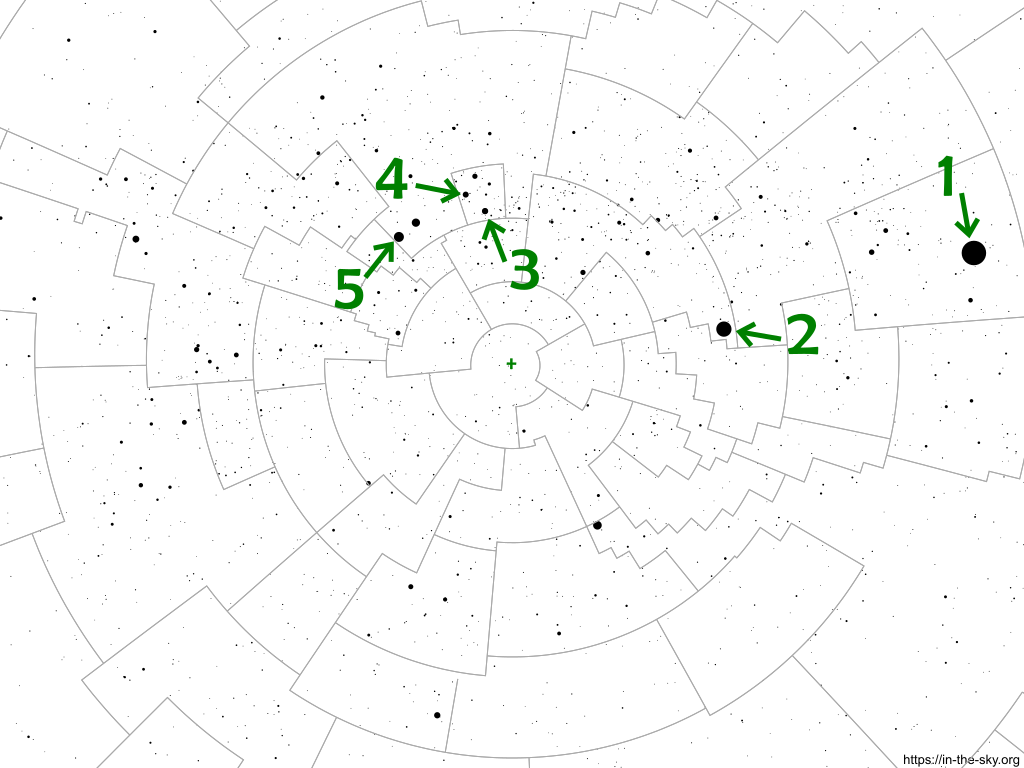
\includegraphics[scale=0.5]{./img/2.png}
			\end{figure}
			\begin{itemize}
				\item \textbf{Pergunta 2a) (0,5 ponto) (0,1 cada acerto)} Marque com \textbf{C} (para certo) ou \textbf{E} (para errado) as afirmações seguintes sobre as estrelas indicadas com os números de $1$ a $5$.
					\begin{itemize}
						\item[$(\quad)$] $1$ é a estrela mais brilhante do céu noturno, recebe o nome de \textit{Sírius} e pertence à constelação \textit{Cão Maior}.
						\item[$(\quad)$] $2$ é a segunda estrela mais brilhante do céu noturno, recebe o nome de \textit{Canopus} e pertence à constelação \textit{Cão Menor}.
						\item[$(\quad)$] $3$ é a segunda estrela mais brilhante da constelação \textit{Cruzeiro do Sul} e recebe o nome de \textit{Estrela de Magalhães}.
						\item[$(\quad)$] $4$ é a estrela mais brilhante da constelação \textit{Cruzeiro do Sul} e recebe o nome de \textit{Mimosa}.
						\item[$(\quad)$] $5$ é a estrela mais brilhante da constelação \textit{Centauro} e recebe o nome de \textit{Rigil Kentaurus}.
					\end{itemize}
				\item \textbf{Pergunta 2b) (0,5 ponto)} O ponto $+$ no centro da imagem representa o Polo Celeste Sul. Sabendo disso, na perspectiva da carta, em qual sentido o céu se movimentaria com o passar do tempo?
					\begin{multicols}{2} \begin{itemize}
						\item[$(\quad)$] Sentido horário
						\item[$(\quad)$] Sentido anti-horário
					\end{itemize} \end{multicols}
			\end{itemize}
		
		\item \textbf{Questão 3) (1 ponto)} Observe a imagem abaixo, a qual representa a visão de um observador no Hemisfério Norte:
			\begin{figure}[H]
				\centering
				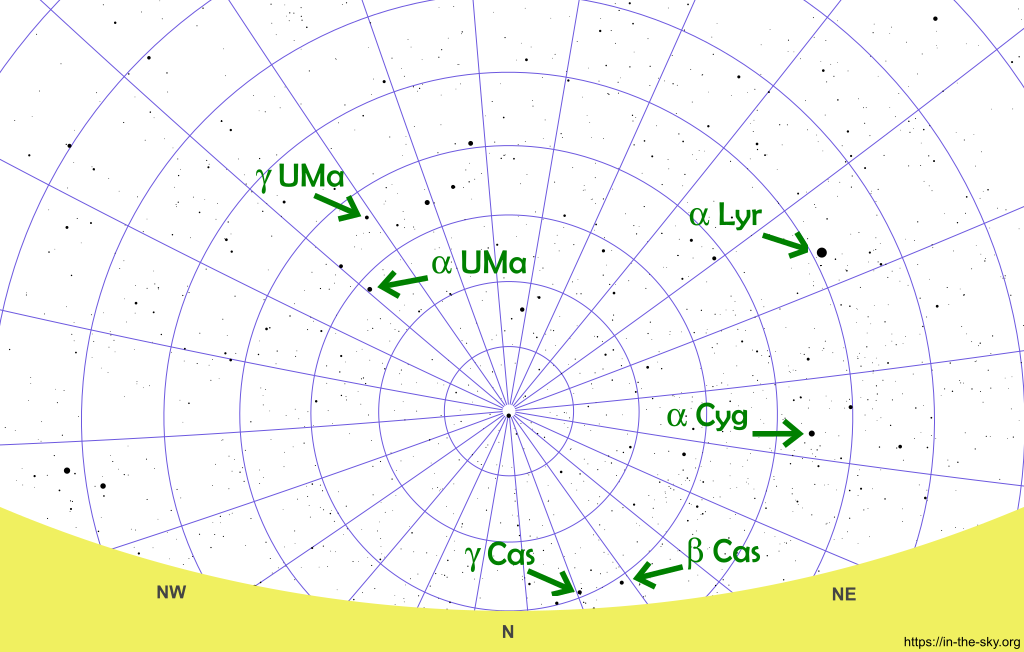
\includegraphics[scale=0.5]{./img/3.png}
			\end{figure}
			em que a cor amarela é o horizonte, o gradiente azul representa o sistema de coordenadas equatoriais, e as anotações em verde foram feitas para facilitar a \textit{Pergunta 3b}, sendo usada a designação de Bayer (letra grega respectiva à posição da estrela na ordem de magnitudes + genitivo da constelação).
			\begin{itemize}
				\item \textbf{Pergunta 3a) (0,4 ponto)} Diferentemente do Hemisfério Sul, o Hemisfério Norte possui uma estrela facilmente reconhecida ao olho nu no Polo Celeste. Essa estrela possui designação de Bayer $\alpha \; UMi$ e é chamada de Polaris. Por estar bem próximo do Polo Celeste, numa fotografia de longa exposição, é possível observar as estrelas se movimentando em sua volta. Sabendo disso, indique a estrela Polaris na imagem acima seguindo o mesmo padrão das anotações em verde (seta + designação de Bayer).
				\item \textbf{Pergunta 3b) (0,6 ponto) (0,1 cada acerto)} Uma estrela é circumpolar se o seu círculo orbital aparente fica totalmente acima do Horizonte. Sabendo disso, marque com as letras $S$ e $N$ as estrelas que são circumpolares e as que não são, respectivamente, na imagem mostrada.
					\begin{multicols}{3} \begin{itemize}
						\item[$(\quad)$] $\alpha$ UMa (Dubhe)
						\item[$(\quad)$] $\gamma$ UMa (Phad)
						\item[$(\quad)$] $\alpha$ Lyr (Vega)
						\item[$(\quad)$] $\alpha$ Cyg (Deneb)
						\item[$(\quad)$] $\beta$ Cas (Caph)
						\item[$(\quad)$] $\gamma$ Cas (Navi)
					\end{itemize} \end{multicols}
			\end{itemize}
			
		\item \textbf{Questão 4) (1 ponto)} Observe a carta celeste seguinte, a qual representa uma região equatorial da Esfera Celeste:
			\begin{figure}[H]
				\centering
				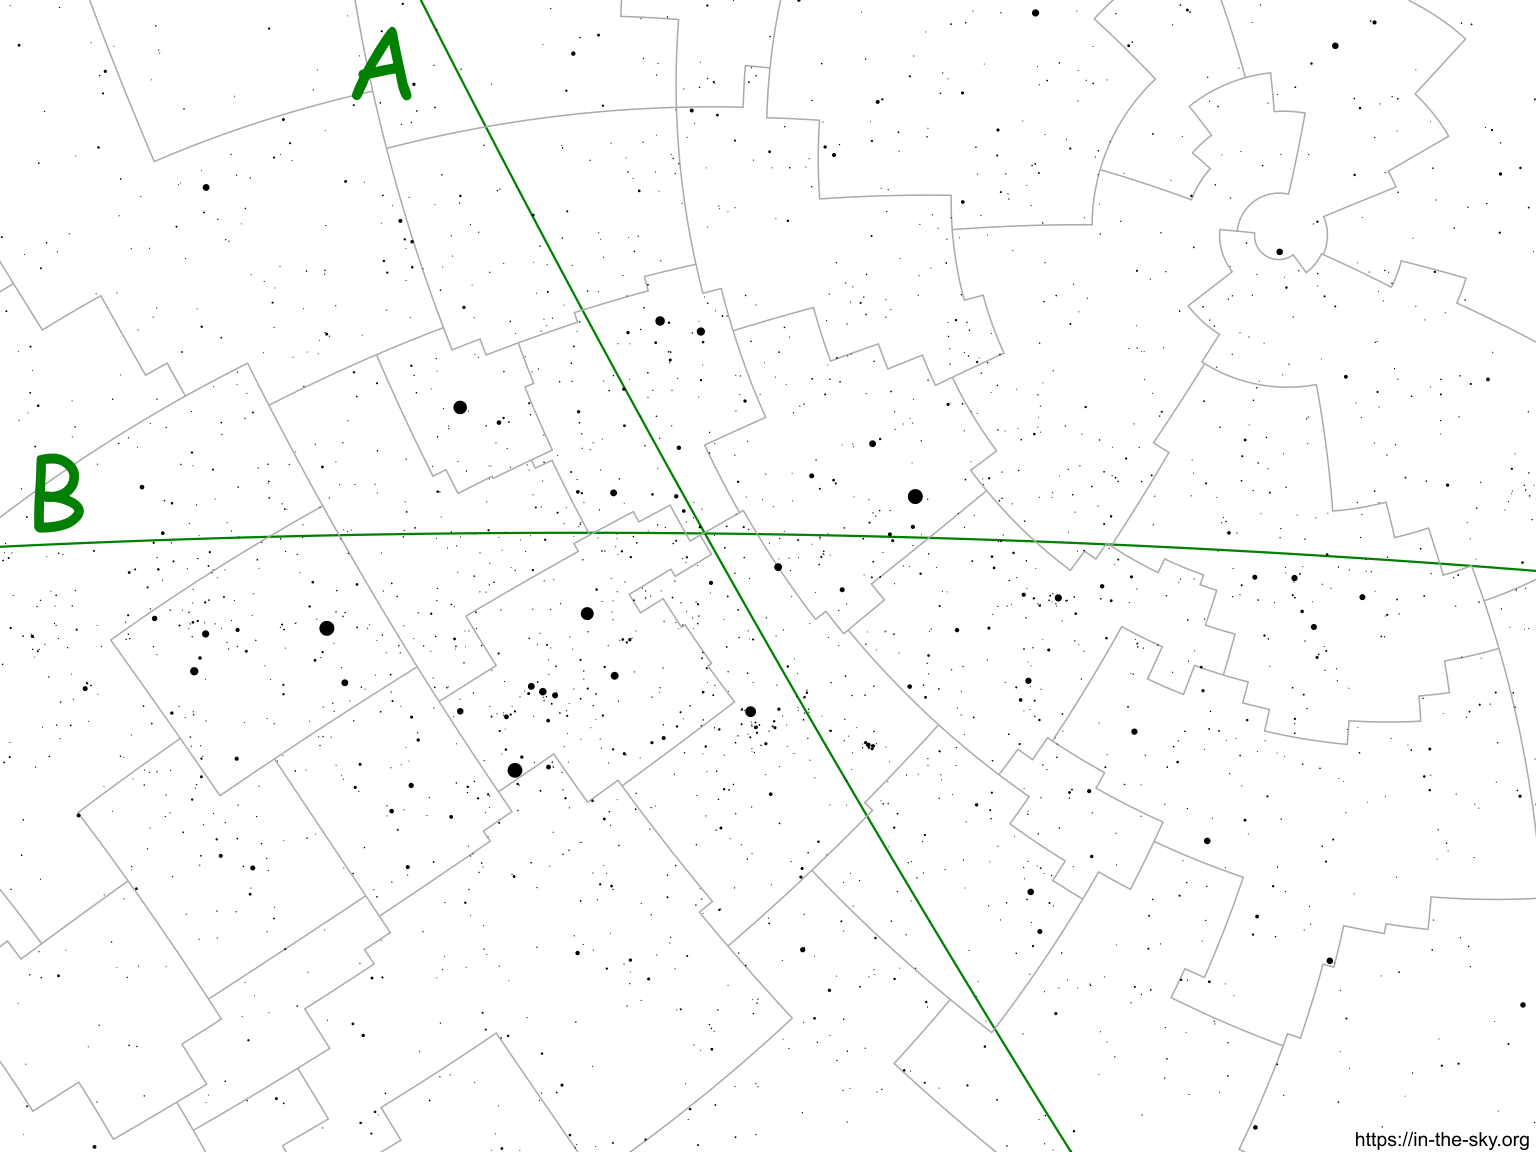
\includegraphics[scale=0.5]{./img/4.png}
			\end{figure}
			em que as linhas cinzas são os limites das constelações e as verdes são planos.
			\begin{itemize}
				\item \textbf{Pergunta 4a) (0,3 ponto)} Indique com um quadrado a posição das estrelas Mintaka, Alnilam e Alnitak, popularmente conhecidas como o Cinturão de Órion ou as Três Marias.
				\item \textbf{Pergunta 4b) (0,3 ponto)} Indique com uma circunferência a posição do aglomerado de estrelas aberto Messier 45, chamado de Plêiades. Esse objeto está na constelação Touro e pode ser encontrado por meio da reta que liga Sírius -- estrela alfa da constelação Cão Maior --, Bellatrix -- estrela gamma da constelação Órion -- e Aldebaran -- estrela alfa da constelação Touro.
				\item \textbf{Pergunta 4c) (0,4 ponto) (0,2 cada acerto)} Abaixo são descritos os caminhos de 3 planos da Esfera Celeste na região ilustrada. Marque com as letras $A$ e $B$ aqueles que podem ser observados na imagem.
					\begin{itemize}
						\item[$(\quad)$] \textit{Plano equatorial:} Hidra Fêmea, Cão Menor, Unicórnio, Órion, Eridano, Touro, e Baleia.
						\item[$(\quad)$] \textit{Plano eclíptico:} Câncer, Gêmeos, Touro, Áries, e Peixes.
						\item[$(\quad)$] \textit{Plano galáctico:} Popa, Cão Maior, Unicórnio, Órion, Touro, Cocheiro, Perseu, Girafa, e Cassiopeia.
					\end{itemize}
			\end{itemize}
				
		\item \textbf{Questão 5) (1 ponto)} Se você tirar uma foto do Sol todos os dia durante 1 ano no mesmo horário e eventualmente fizer uma sobreposição da posição do sol em uma só foto, você terá um formato conhecido como \textit{Analema}.
			\begin{itemize}
				\item \textbf{Pergunta 5a) (0,5 ponto)} Marque a(s) imagem(s) abaixo que representam formatos possíveis para um analema.
					\begin{multicols}{2}
						\begin{figure}[H]
							\centering
							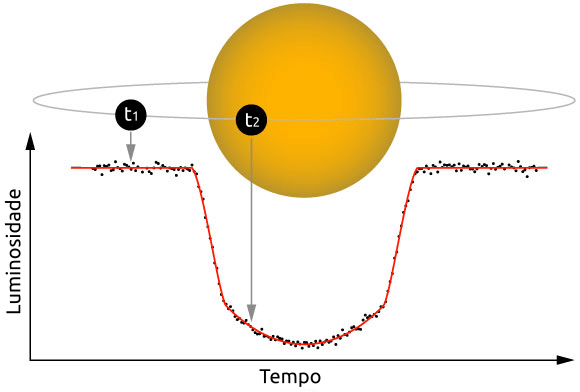
\includegraphics[scale=0.15]{./img/5a}
							\captionsetup{labelformat=empty}
							\caption{$(\quad)$}
						\end{figure}
						\begin{figure}[H]
							\centering
							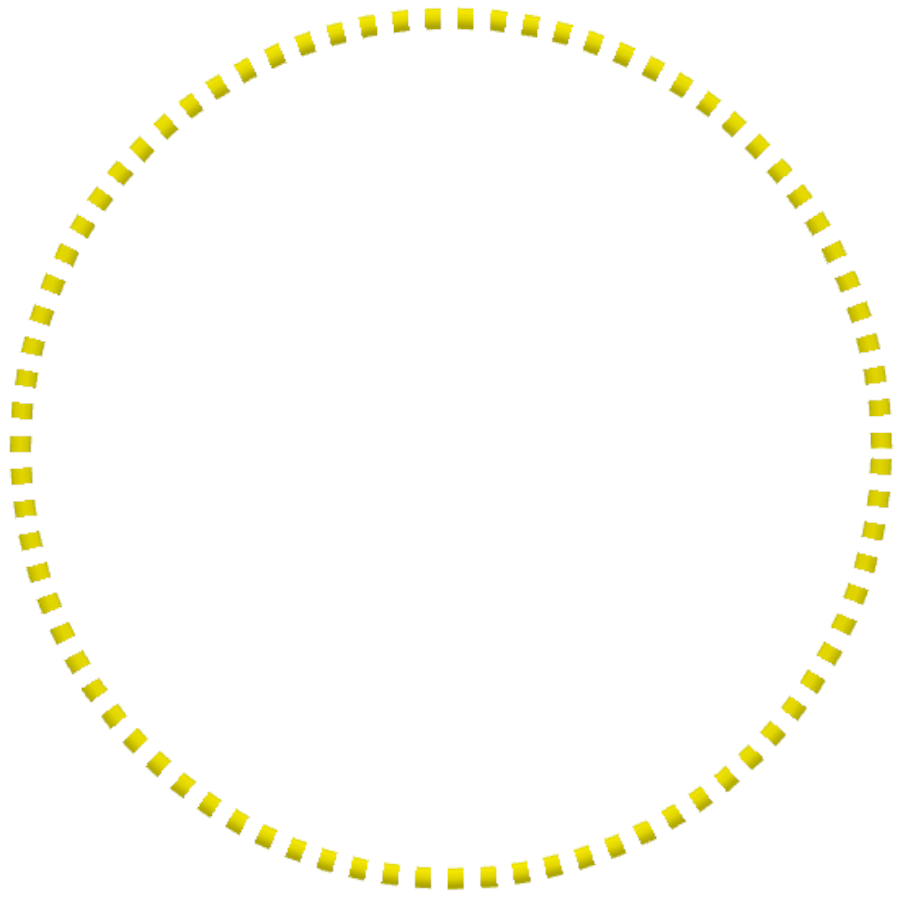
\includegraphics[scale=0.15]{./img/5b}
							\captionsetup{labelformat=empty}
							\caption{$(\quad)$}
						\end{figure}
						\begin{figure}[H]
							\centering
							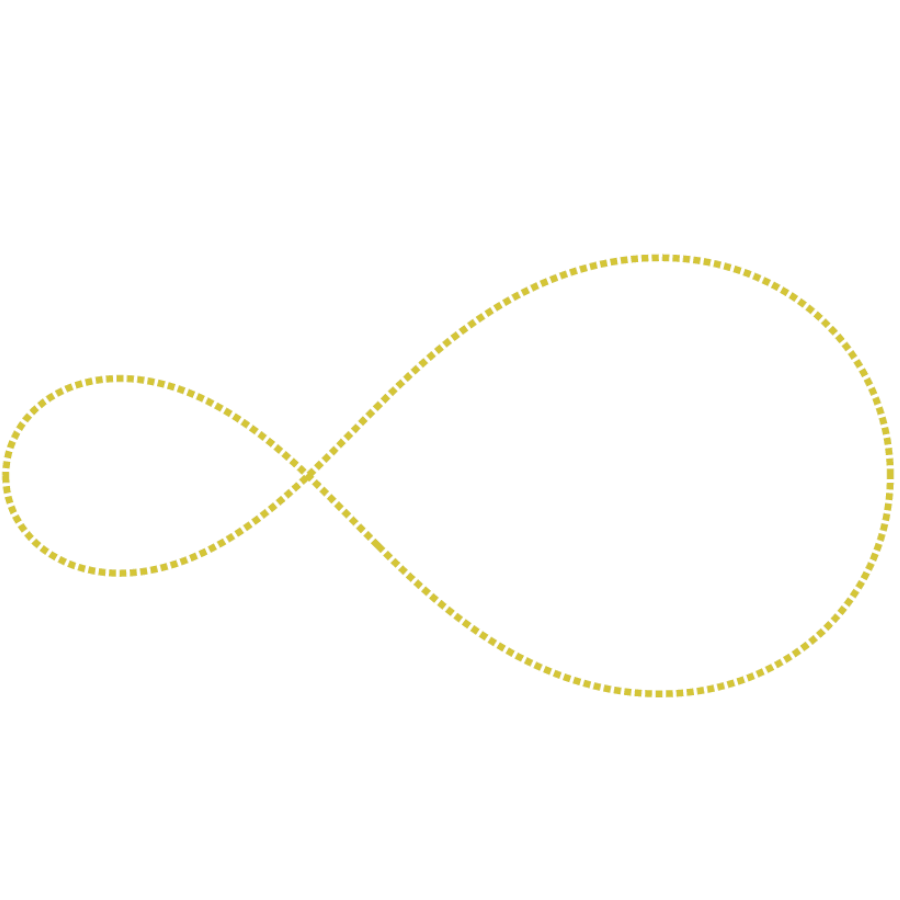
\includegraphics[scale=0.15]{./img/5c}
							\captionsetup{labelformat=empty}
							\caption{$(\quad)$}
						\end{figure}
						\begin{figure}[H]
							\centering
							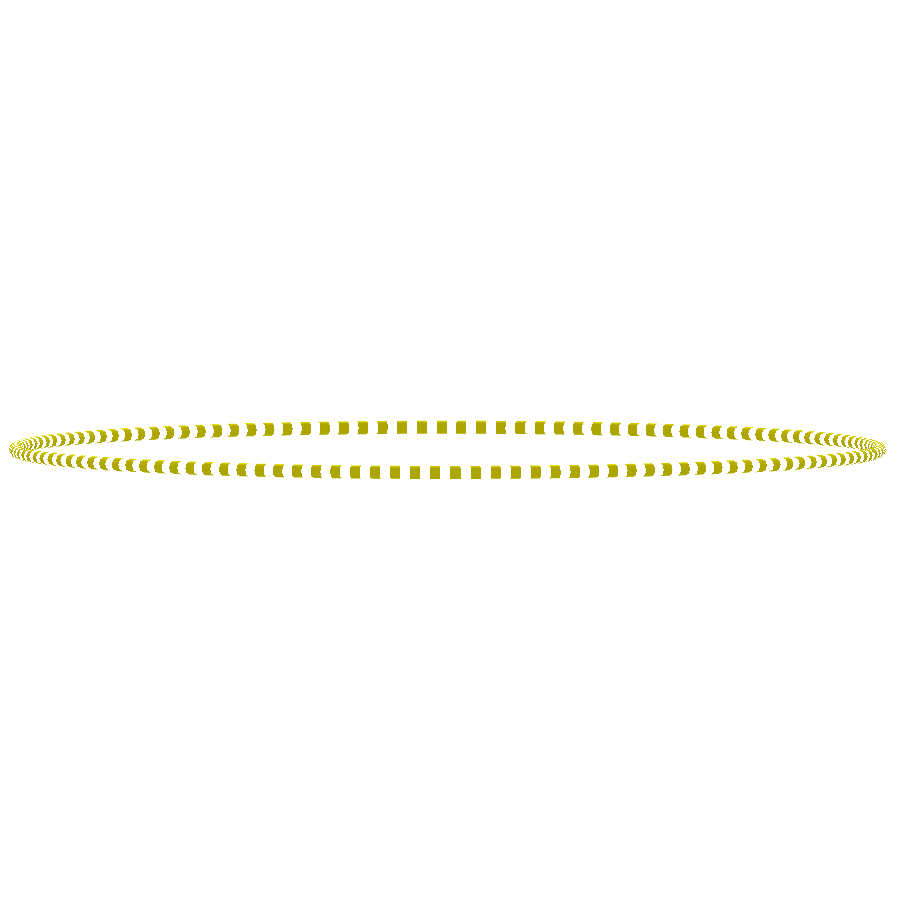
\includegraphics[scale=0.15]{./img/5d}
							\captionsetup{labelformat=empty}
							\caption{$(\quad)$}
						\end{figure}
					\end{multicols}
				\item \textbf{Pergunta 5b) (0,5 ponto)} Marque o(s) fator(es) abaixo que possuem grande influência nos formatos possíveis de um analema.
					\begin{itemize}
						\item[$(\quad)$] Inclinação entre o Equador Celeste e a Eclíptica.
						\item[$(\quad)$] Rotação terrestre.
						\item[$(\quad)$] Translação terrestre ao redor do Sol.
						\item[$(\quad)$] Formato elíptico da órbita terrestre.
						\item[$(\quad)$] Precessão dos Equinócios
					\end{itemize}
			\end{itemize}
			
	\end{itemize}
	\end{flushleft}
	\begin{flushright}
		\begin{large}
			Bons estudos!
		\end{large}
	\end{flushright}
\end{document}